%!TEX root = ../thesis.tex
% ******************************* Thesis Appendix E ********************************

\chapter{GEANT4 Light Output Vs. Fitted Light Output}

\begin{figure}[htbp]
\centering
\begin{subfigure}{.5\textwidth}
  \centering
  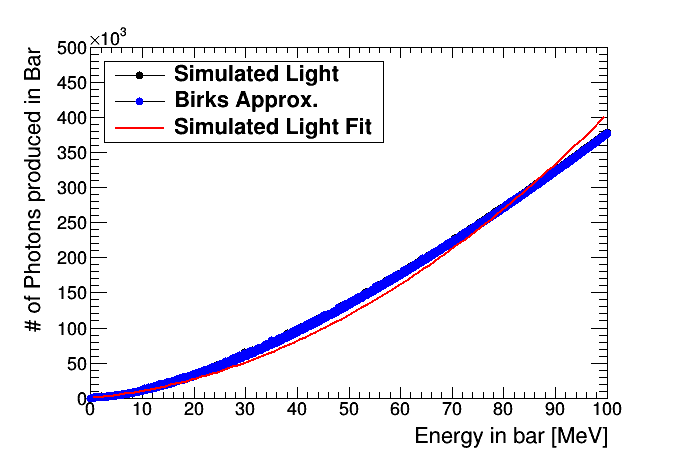
\includegraphics[width=\linewidth]{Appendix5/Figs/light_of_Alphas0-100mev.png}
  \captionsetup{width=.9\linewidth}
  \caption{Simulated 1E6 $\alpha$ particles.}
  \label{subfig:append5_light_of_Alphas0-100mev}
\end{subfigure}
\begin{subfigure}{.5\textwidth}
  \centering
  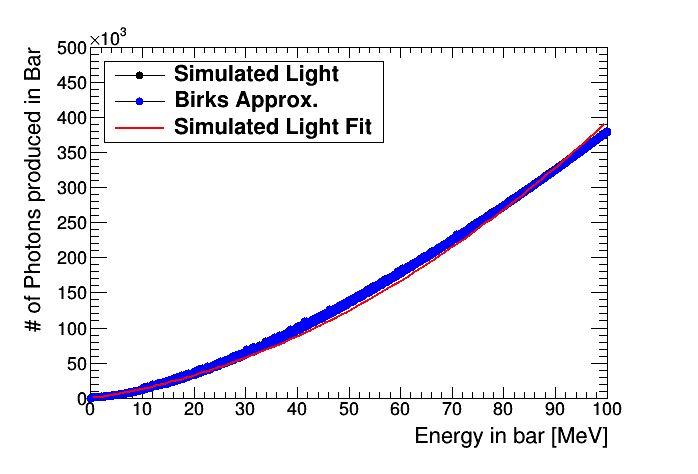
\includegraphics[width=\linewidth]{Appendix5/Figs/light_of_AAlphas0-100mev.png}
  \captionsetup{width=.9\linewidth}
  \caption{Simulated 1E6 $\bar{\alpha}$ particles.}
  \label{subfig:append5_light_of_AAlphas0-100mev}
\end{subfigure}
\caption{How the Birk's approximation (equation \ref{equ:Birks_formula}) approximates light for alpha particles. The Birk's approximation is very suitable for these particles.}
\label{fig:append5_light_of_Alphas_AAlphas0-100mev}
\end{figure}

\begin{figure}[htbp]
\centering
\begin{subfigure}{.5\textwidth}
  \centering
  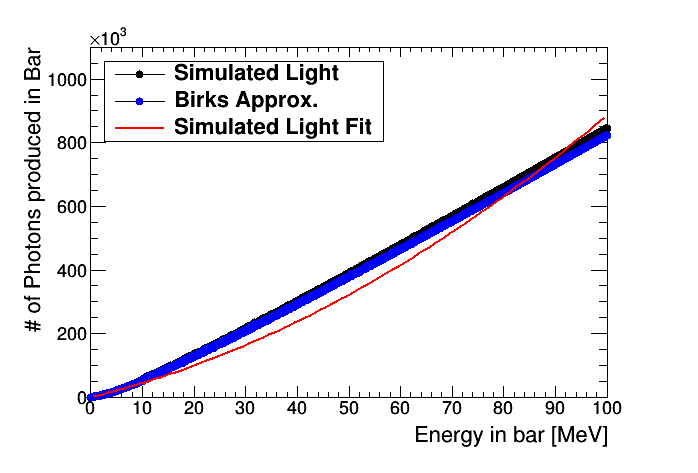
\includegraphics[width=\linewidth]{Appendix5/Figs/light_of_protons0-100mev.png}
  \captionsetup{width=.9\linewidth}
  \caption{Simulated 1E6 proton particles.}
  \label{subfig:append5_light_of_protons0-100mev}
\end{subfigure}%
\begin{subfigure}{.5\textwidth}
  \centering
  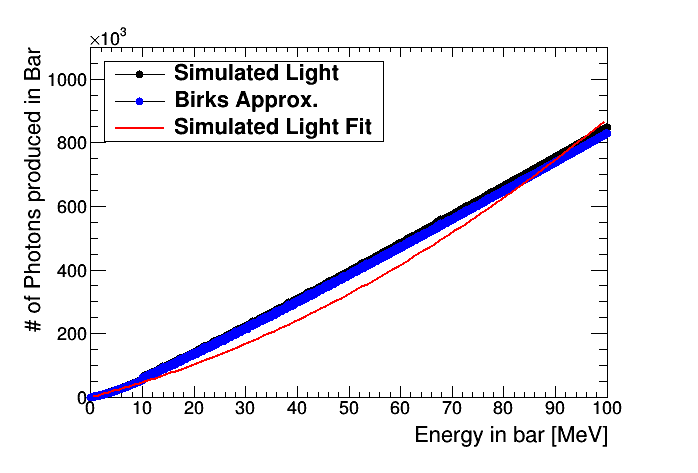
\includegraphics[width=\linewidth]{Appendix5/Figs/light_of_Aprotons0-100mev.png}
  \captionsetup{width=.9\linewidth}
  \caption{Simulated 1E6 anti-proton particles.}
  \label{subfig:append5_light_of_Aprotons0-100mev}
\end{subfigure}
\caption{How the Birk's approximation (equation \ref{equ:Birks_formula}) approximates light for protons and anti-protons. The Birk's approximation is very suitable for these particles.}
\label{fig:append5_light_of_protons_Aprotons0-100mev}
\end{figure}

\begin{figure}[htbp]
\centering
\begin{subfigure}{.5\textwidth}
  \centering
  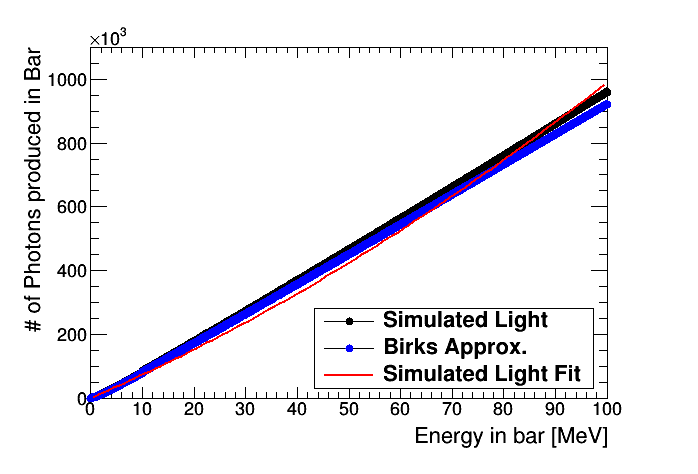
\includegraphics[width=\linewidth]{Appendix5/Figs/light_of_pIPlus0-100mev.png}
  \captionsetup{width=.9\linewidth}
  \caption{Simulated 1E6 $\pi^+$ particles.}
  \label{subfig:append5_light_of_pIPlus0-100mev}
\end{subfigure}%
\begin{subfigure}{.5\textwidth}
  \centering
  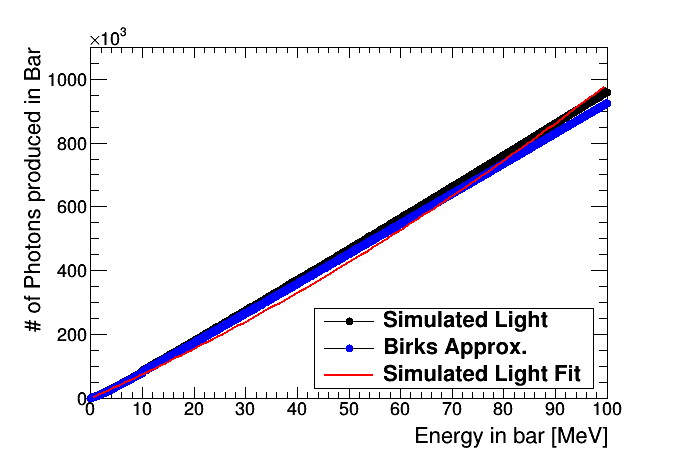
\includegraphics[width=\linewidth]{Appendix5/Figs/light_of_pIMinus0-100mev.png}
  \captionsetup{width=.9\linewidth}
  \caption{Simulated 1E6 $\pi^-$ particles.}
  \label{subfig:append5_light_of_pIMinus0-100mev}
\end{subfigure}
\caption{How the Birk's approximation (equation \ref{equ:Birks_formula}) approximates light for $\pi^+$ and $\pi^-$. The Birk's approximation is suitable between 0\,MeV -- 60\,MeV. Above 60\,MeV there is a slight discrepancy between the Birk's approximation and GEANT4 simulated values. Birk's approximation is still used.}
\label{fig:append5_light_of_pIPlus_pIMinus0-100mev}
\end{figure}

\begin{figure}[htbp]
\centering
\begin{subfigure}{.5\textwidth}
  \centering
  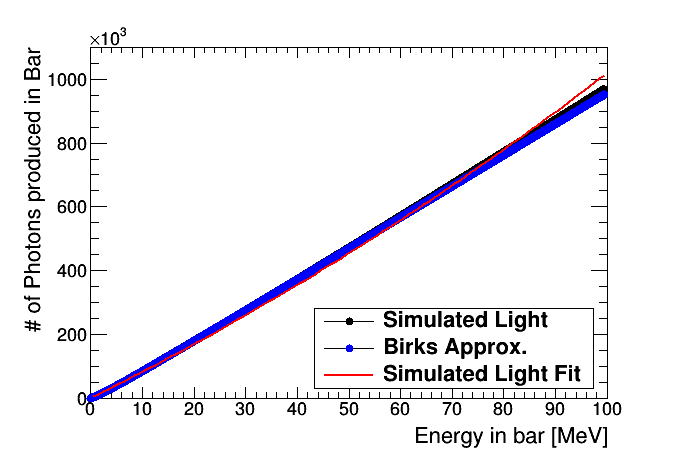
\includegraphics[width=\linewidth]{Appendix5/Figs/light_of_muons0-100mev.png}
  \captionsetup{width=.9\linewidth}
  \caption{Simulated 1E6 $\mu^-$ particles.}
  \label{subfig:append5_light_of_muons0-100mev}
\end{subfigure}%
\begin{subfigure}{.5\textwidth}
  \centering
  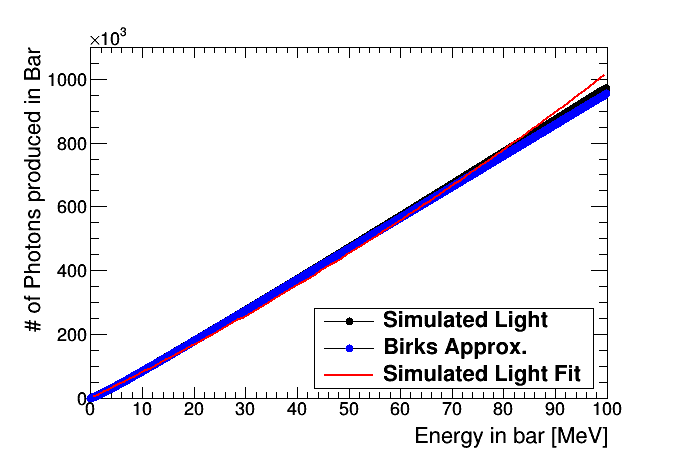
\includegraphics[width=\linewidth]{Appendix5/Figs/light_of_Amuons0-100mev.png}
  \captionsetup{width=.9\linewidth}
  \caption{Simulated 1E6 $\mu^+$ particles.}
  \label{subfig:append5_light_of_Amuons0-100mev}
\end{subfigure}
\caption{How the Birk's approximation (equation \ref{equ:Birks_formula}) approximates light for $\mu^-$ and $\mu^+$. The Birk's approximation is very suitable for these particles.}
\label{fig:append5_light_of_muons_Amuons0-100mev}
\end{figure}

\begin{figure}[htbp]
\centering
\begin{subfigure}{.5\textwidth}
  \centering
  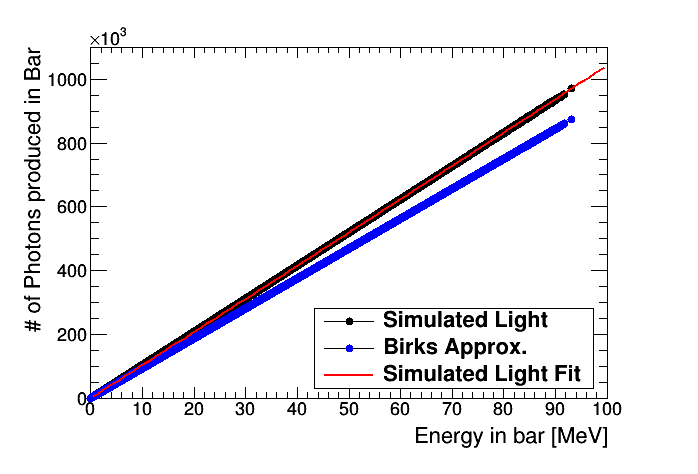
\includegraphics[width=\linewidth]{Appendix5/Figs/light_of_electrons0-100mev.png}
  \captionsetup{width=.9\linewidth}
  \caption{Simulated 1E6 $e^-$ particles.}
  \label{subfig:append5_light_of_electrons0-100mev}
\end{subfigure}%
\begin{subfigure}{.5\textwidth}
  \centering
  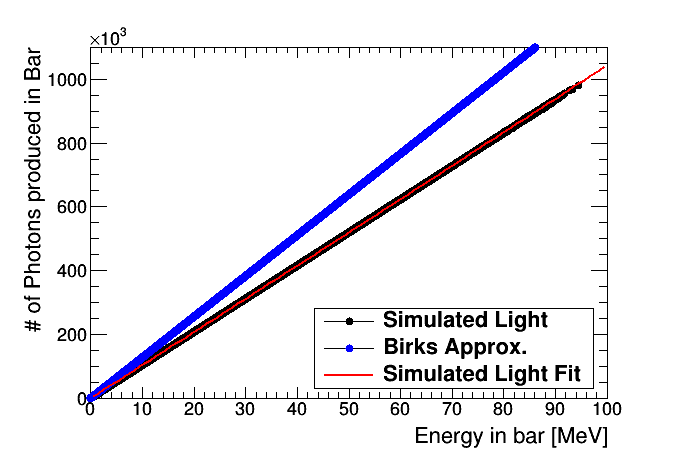
\includegraphics[width=\linewidth]{Appendix5/Figs/light_of_positrons0-100mev.png}
  \captionsetup{width=.9\linewidth}
  \caption{Simulated 1E6 $e^+$ particles.}
  \label{subfig:append5_light_of_positrons0-100mev}
\end{subfigure}
\caption{How the Birk's approximation (equation \ref{equ:Birks_formula}) approximates light for e$^-$ and $e^+$. The Birk's approximation is unsuitable here especially for $e^+$ which are breaking the conservation of energy.}
\label{fig:append5_light_of_electrons_positrons0-100mev}
\end{figure}

\begin{figure}[htbp]
\centering
\begin{subfigure}{.5\textwidth}
  \centering
  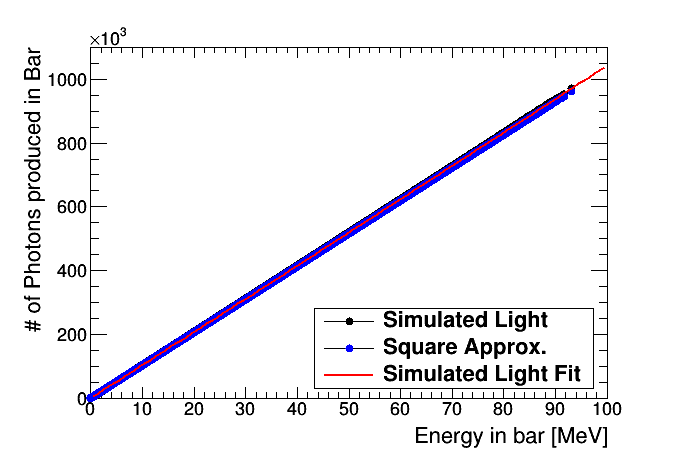
\includegraphics[width=\linewidth]{Appendix5/Figs/light_of_electronsLin0-100mev.png}
  \captionsetup{width=.9\linewidth}
  \caption{Simulated 1E6 $e^-$ particles.}
  \label{subfig:append5_light_of_electronsLin0-100mev}
\end{subfigure}%
\begin{subfigure}{.5\textwidth}
  \centering
  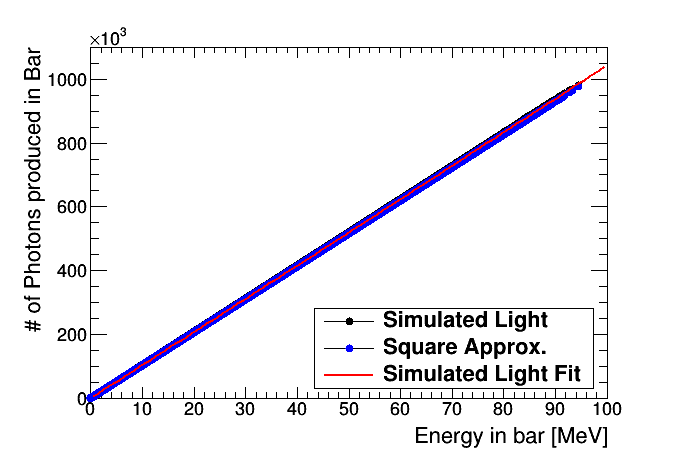
\includegraphics[width=\linewidth]{Appendix5/Figs/light_of_positronsLin0-100mev.png}
  \captionsetup{width=.9\linewidth}
  \caption{Simulated 1E6 $e^+$ particles..}
  \label{subfig:append5_light_of_positronsLin0-100mev}
\end{subfigure}
\caption{How the square function approximates light for e$^-$ and $e^+$. This approximation is suitable approximation of the GEANT4 light output.}
\label{fig:append5_light_of_electrons_positronsLin0-100mev}
\end{figure}